%
% green-curve.tex
%
% (c) 2018 Prof Dr Andreas Müller, Hochschule Rapperswil
%
\documentclass[tikz]{standalone}
\usepackage{times}
\usepackage{txfonts}
\usepackage[utf8]{inputenc}
\usepackage{graphics}
\usepackage{ifthen}
\usepackage{color}
\usetikzlibrary{arrows,intersections}
\begin{document}


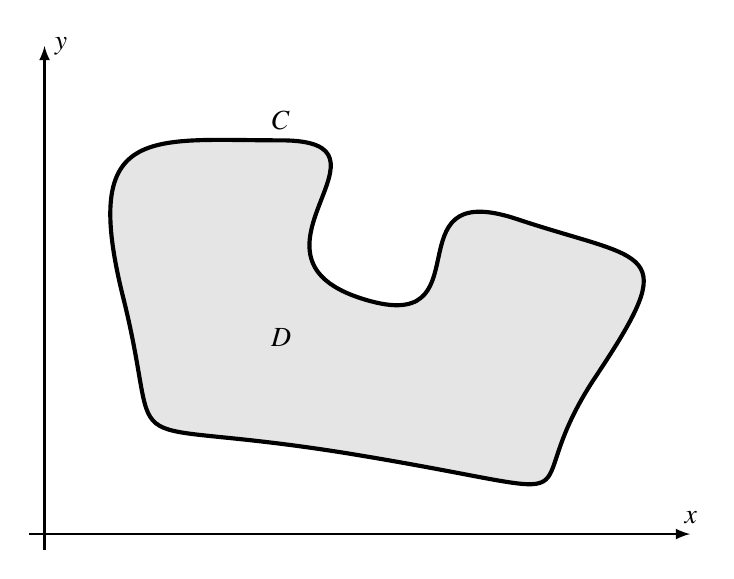
\begin{tikzpicture}[thick, >= latex]

\coordinate (O) at (0,0);

\draw[->] (-0.2,0)--(8.2,0) coordinate[label={above:$x$}];
\draw[->] (0,-0.2)--(0,6.2) coordinate[label={right:$y$}];

\fill[color=gray!20] plot [smooth cycle,tension=2]
coordinates { (1,3) (4,1) (7,2) (6,4) (4,3) (3,5) };

\draw[line width=1.5pt] plot [smooth cycle,tension=2]
coordinates { (1,3) (4,1) (7,2) (6,4) (4,3) (3,5) };

%\draw (1,3) circle[radius=0.1];
%\draw (4,1) circle[radius=0.1];
%\draw (7,2) circle[radius=0.1];
%\draw (6,4) circle[radius=0.1];
%\draw (4,3) circle[radius=0.1];
%\draw (3,5) circle[radius=0.1];

\node at (3,5) [above] {$C$};

\node at (3,2.5) {$D$};

\end{tikzpicture}
\end{document}

